\chapter{Solution approach} \label{chap:solution-apporach}

\todo{%
We design two algorithms to identify and relax bottlenecks in the \ac{rcpsp}.
The first algorithm utilizes identification indicators to identify bottleneck machines
and by processing the machine load function,
periods for potential resource capacity relaxations are found.
For this purpose, we adapt existing Job-Shop bottleneck identification indicators
for the use in the \ac{rcpsp}.
The second algorithm generates partial solutions by considering time-variable relaxations
and proposes relaxations to the original problem based on solutions to the relaxed problems.
}

% ~~~~~~~~~~~~~~~~~~~~~~~~~~~~~~~~~~~~~~~~~~~~~~~~~~~~~~~~~~~~~~~~~~~~~~~~~~~~~~~~~~~~~~~~~~~~~~~~~~~~~~~~~~~
\section{Baseline solution} \label{sec:solution-apporach/baseline-solution}

\todo{Intro}

% -----------------------------------------------------------------------------------------------------------
\subsection{Adapted identification indicators}

We adapt existing identification indicators to detect bottlenecks,
specifically the \acf{mur} and \acf{auad} indicators.
(For definitions, see \cref{subsec:related-works/bottlenecks-in-scheduling/identification-indicators}.)
        
The \ac{mur}, first utilized as a bottleneck identification indicator by \citet{Lawrence1994},
considers the ratio of executed work on a resource to the total time the resource was used.
Despite its simplicity, the \ac{mur} indicator has proven effective at identifying long-run bottlenecks.
(Long-run bottlenecks could be viewed as structural bottlenecks ---
see \cref{subsec:related-works/bottlenecks-in-scheduling/bottleneck-classification} for bottleneck classification).

The \ac{auad}, initially proposed by \citet{Roser2001},
is slightly more complex but remains a comprehensive indicator for identifying bottleneck resources.
For the specified resource, the sequence of all uninterrupted execution periods is computed
and the average length of those periods is considered the indicator value.
An uninterrupted period is a sequence of jobs scheduled consecutively with no idle times between them.
If there is an idle time period between two subsequent jobs,
they belong to different uninterrupted periods.

Both identification indicators consider the relationship between the total duration
of job executions on a resource and the duration for which the resource is idle.
In a Job-Shop scheduling problem,
this represents all the available information.
This concept remains applicable in the \ac{rcpsp}.
However, due to the variability of machine load over time in the \ac{rcpsp},
a binary \enquote{processing-idle} differentiation between machine states
does not provide a sufficient machine-load indication.
In the \ac{rcpsp}, we have additional information available.
By incorporating resource capacities and resource consumptions into the calculation,
we can achieve a more precise result that better corresponds to the actual machine load.
\cref{fig:MachineLoad} illustrates the difference in variability of the load between
a Job-Shop machine (subfigure \ref{fig:MachineLoad:JS})
and a \ac{rcpsp} machine (subfigure \ref{fig:MachineLoad:RCPSP}).

\begin{figure}[t]
    \centering
    
    \subfloat[Job Shop]{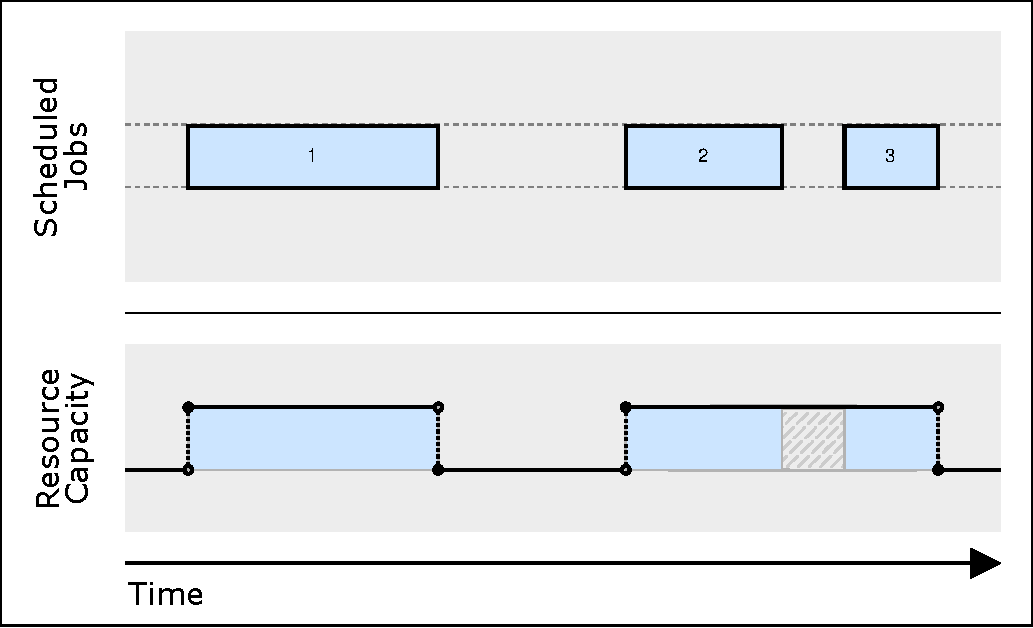
\includegraphics[width=0.7\textwidth]{img/Capacities-JobShop.pdf}\label{fig:MachineLoad:JS}}
    \\
    \subfloat[RCPSP]{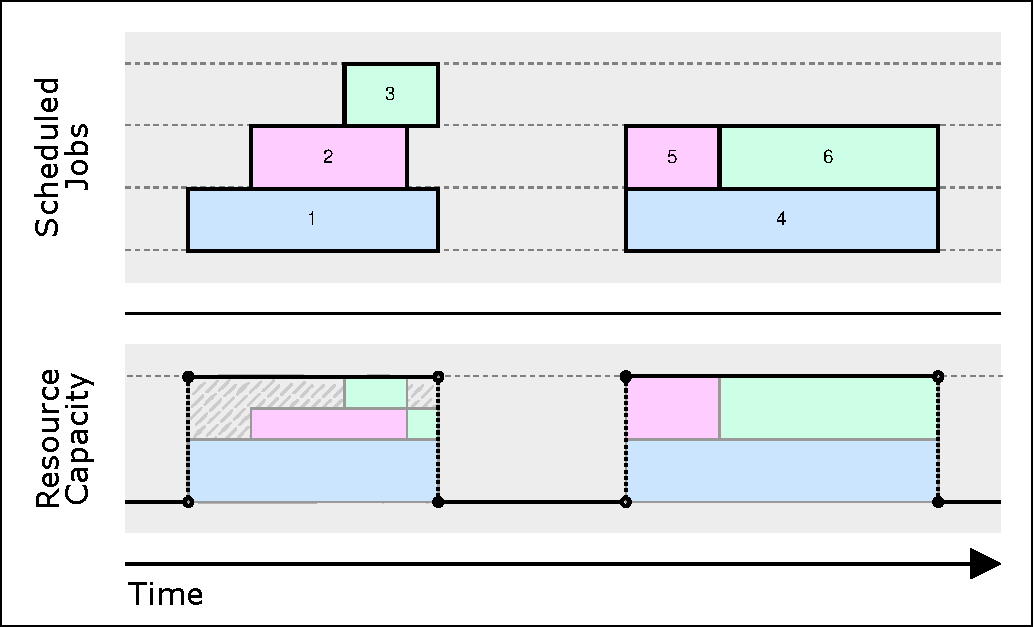
\includegraphics[width=0.7\textwidth]{img/Capacities-RCPSP.pdf}\label{fig:MachineLoad:RCPSP}}
    
    \caption{
        Examples of machine-load functions of the Job-Shop problem and the \ac{rcpsp} problem.
        The variability in the possible machine loads during job execution
        between the Job-Shop problem and the \ac{rcpsp}
        and the variability in machine loads during different periods in the \ac{rcpsp} are demonstrated.
        }
    \label{fig:MachineLoad}
\end{figure}

We propose \acf{mrur} as the adaptation of \ac{mur} and \acf{auau} as the adaptation of \ac{auad}.
For a resource $k$, the \ac{mrur} is defined as:
$$
\indMRUR{k} \defeq \frac{\sum_{j \in \Jobs} (\duration{j} \cdot \consumption{j}{k})}%
                        {\sum_{t=1}^{C_{\max}} \capacity{k}{t}},
$$
where $C_{\max} \defeq \max_{j \in \Jobs} \jobend{j}$%
\footnote{In scheduling literature,
$C_{\max}$ is referred to as the \emph{makespan} of the project.
Minimizing project makespan is a common optimization goal in scheduling,
and it is a simpler alternative to the total weighted tardiness we use.}.
For a resource $k$, the \ac{auau} is defined as:
$$
\indAUAU{k} \defeq \frac{\sum_{i=1}^{A_k} \indPRU{k}{i}}%
                        {A_k},
$$
where the \acf{pru} of resource $k$ during the uninterrupted active period $i$
is defined as
$$
\indPRU{k}{i} \defeq \frac{\sum_{j \in \JobsOnResourceInPeriod{k}{i}}
                                \duration{j} \cdot \consumption{j}{k}}%
                          {\sum_{t=a_{ki}^{S}}^{a_{ki}^{E}} \capacity{k}{t} }.
$$
For a resource $k$,
$(a_{k1}^{S}, a_{k1}^{E}), \dots, (a_{kA_k}^{S}, a_{kA_k}^{E})$
is the the sequence of \emph{uninterrupted active periods},
where $a_{ki}^{S} \in \intinterval{1}{\horizon}$ denotes the start of the period $i$
and $a_{ki}^{E} \in \intinterval{1}{\horizon}$ denotes the end of the period $i$.
\toask{% JE TOTO ROZUMNÁ DEFINICE?
Similar to the definition of \ac{auad} but with differences induced by non-unit capacities,
an uninterrupted active period is a maximal set (maximal in terms of inclusion)
of jobs scheduled consecutively or in parallel with no idle time
occurring on the considered resource during the period.
Two jobs are in the same uninterrupted active period, if and only if
the execution intervals of the jobs overlap
or the considered resource is not idle between the execution intervals of the jobs.
The sequence of uninterrupted active periods of a resource is the transitive closure of this relation
on jobs executed on the resource.
}
Here, as opposed to the \ac{auad},
we consider not the duration of the periods,
but the individual jobs executed during each of the periods,
specifically their durations and consumptions of the evaluated resource.

In the formula for $\indPRU{k}{i}$,
$\JobsOnResourceInPeriod{k}{i} \defeq \{ j \in \JobsOnResource{k} : a_{ki}^{S} \leq \jobstart{j} \leq a_{ki}^{E} \}$
is the set of jobs executed on resource $k$ during the uninterrupted active period $i$.
(Recall from \cref{subsec:related-works/bottlenecks-in-scheduling/identification-indicators} that
$\JobsOnResource{k} = \{ j \in \Jobs : \consumption{j}{k} > 0 \}$.)

Having proposed bottleneck identification indicators for our \ac{rcpsp} variant,
we will formulate an algorithm utilizing those indicators in the following section.

% -----------------------------------------------------------------------------------------------------------
\subsection{Identification indicator-based relaxing algorithm}

In this section, we formulate the \acf{iira}.
\ac{iira} employs a specified bottleneck identification indicator to identify bottleneck resources.
It calculates the granular resource load
and uses convolution to determine the improvement potential for granular periods.
Finally, it relaxes capacity constraints in granular periods with the greatest improvement potential.
Following this, a solution is obtained for the relaxed problem instance,
and the proposed capacity relaxations are reduced to only include those utilized by the new solution.
We will now formulate the algorithm in \cref{alg:identification-indicator-relaxing-algorithm}.

\begin{algorithm}[t]
\caption{\acl{iira}}
\label{alg:identification-indicator-relaxing-algorithm}
\begin{algorithmic}[1]

\Params  Identification indicator $\algIndicator$, granularity $\algGranularity$, convolution mask $\algConvolution$,
\Paramsc iterations limit $\algMaxiter$, improvement periods limit $\algMaxperiods$,
\Paramsc capacity improvement $\algImprovement$
\Input  Solution $\Schedule$ to a problem instance $\Instance$

\State $PC \gets \lceil \horizon / \algGranularity \rceil$
       \Comment The number of granular periods
\State $\Instance^* \gets \Instance$, $\Schedule^* \gets \Schedule$
       \Comment Modified instance and its solution, initially
       \Statecr copies of the original instance and solution
\Repeat
    \State Evaluate $\Schedule^*$ using $\algIndicator$, obtaining:
           $\algIndicator_k \;\forall k \in \Resources$
    \State Identify bottleneck resource:
           $k^* \gets \argmax_k \algIndicator_k$
    \State Compute granular resource load for $k^*$:
    \Statec{3} $\resourceLoad{k^*} \gets $ \Callref{GranularResourceLoad}%
                                                   {$k^*$, $\Instance^*$, $\Schedule^*$, $PC$}%
                                                   {alg:granular-resource-load}
    \State Compute improvement potential of periods: $\Psi \gets \resourceLoad{k^*} * \algConvolution$
    \State Find improvement periods:
    \Statec{3} $p_1, \dots, p_{\algMaxperiods} \gets$
            periods with the highest potential $\Psi(i)$
    \For {$i \gets p_1, \dots, p_{\algMaxperiods}$}
        \State $\capacityf{k^*}^* \gets$ \Callref{IncreaseGranularPeriodCapacity}%
                                                 {$i$, $\capacityf{k^*}^*$, $\algGranularity$, $\algImprovement$}%
                                                 {alg:increase-granular-period-capacity}
    \EndFor
    \State Find solution $\Schedule^*$ to the modified instance $\Instance^*$
    \State $\capacityf{k^*}^* \gets$ \Callref{ReduceCapacityChanges}%
                                             {$k$, $\capacityf{k^*}$, $\Instance^*$, $\Schedule^*$}%
                                             {alg:reduce-capacity-changes}
    \State $\Additions^{\Instance^*}, \Migrations^{\Instance^*} \gets $
           \Callref{FindAdditionsAndMigrations}%
                   {$\capacityf{k^*}^*$, $\Instance^*$, $\Schedule^*$}%
                   {alg:find-additions-and-migrations}
\ForIter{$\algMaxiter$}

\Output Modified instance $\Instance$ and its solution $\Schedule^*$

\Note In the call to \Call{ReduceCapacityChanges}{} (statement 12),
      $\capacityf{k^*}$ from the~original instance is given as the original capacity function of the resource $k^*$.
\end{algorithmic}
\end{algorithm}

The algorithm statement contains the use of multiple utility functions and procedures.
To maintain brevity,
we exclude the detailed specifics of the procedures and instead offer a short overview of each procedure.
Complete statements of the procedures are available in \cref{sec:attachments/algorithms-functions-procedures}.

\begin{itemize}
    \item \algnameref{GranularResourceLoad}{alg:granular-resource-load}
        computes a granular resource load for a given resource.
        The granular load is a function mapping granular periods to the cumulative sum of the load
        of the resource over the specified granular period.
        
    \item \algnameref{IncreaseGranularPeriodCapacity}{alg:increase-granular-period-capacity}
        increases the values of the given capacity function during the specified granular period.
        The capacity is increased in each time period covered by the granular period,
        determined by the specified granularity.

    \item \algnameref{ReduceCapacityChanges}{alg:reduce-capacity-changes}
        constructs a reduced capacity function for the given resource based on the original resource function
        and the actual load of the resource (computed from the given solution).
        This function reduces redundant capacity additions introduced by former relaxations,
        so that the resource capacity function does not contain capacity additions not utilized by the solution.

    \item \algnameref{FindAdditionsAndMigrations}{alg:find-additions-and-migrations}
        finds capacity additions and migrations (as defined in \cref{sec:problem-statement/alternative-schedule}).
        First, capacity migrations are computed to utilize existing capacities in the given problem instance.
        Then, when no other migrations are possible, the remaining capacity addition requirements are fulfilled
        by introducing capacity additions.

\end{itemize}

\todo{REVISION of algorithms}

% ~~~~~~~~~~~~~~~~~~~~~~~~~~~~~~~~~~~~~~~~~~~~~~~~~~~~~~~~~~~~~~~~~~~~~~~~~~~~~~~~~~~~~~~~~~~~~~~~~~~~~~~~~~~
\section{Extended solution} \label{sec:solution-apporach/extended-solution}

We propose a procedure which detects bottlenecks in the schedule and relaxes those bottlenecks to obtain
an improved schedule.

\begin{itemize}
    \item 

    \item Apply the method to identify bottlenecks
    \item Relax bottlenecks --- one by one, combined?
    \item Propose alternative solutions
    \begin{itemize}
        \item Extremal solutions based on some similarity/improvement metrics?
        \item Scalable solution?
    \end{itemize}
\end{itemize}

The procedure:

\begin{steps}
    \item Find intervals to relax. \label{enum:procedureStart}
    \item Relax proposed intervals --- migrate capacities where possible; otherwise add new capacities.
    \item Find a solution to the modified problem.
    \item Reduce capacity changes to only include the utilized changes.
    \item Repeat from \cref{enum:procedureStart} for predefined number of iterations.
\end{steps}

Find intervals to relax:

\begin{verbatim}
For $i in j$
\end{verbatim}


\begin{algorithm}
\begin{algorithmic}
\Function{FindIntervalsToRelax}{}
	\State $r \gets$ a random number between $0$ and $1$
	\State $\varepsilon \gets 0.0000000000000000000000000000000000000042$
	\If{$r\geq\varepsilon$}
		\State execute $A$ \Comment{We discard the return value}
	\Else
		\State print: \texttt{Not today, sorry.}
        \EndIf


    \State $a$
\EndFunction
\end{algorithmic}
\caption{TODO}
\label{alg:findIntervalsToRelax}
\end{algorithm}
 